% Provenance (never printed): see sources/outline_sources.md (Year 1:
% the Solar System, planetology). Kepler's laws, the moment of inertia and
% the Stefan--Boltzmann law are owned by the physics series and recalled
% here; the equilibrium temperature and the Bond albedo are re-founded from
% Book 2 grade 10. Curves computed in figdata/bachelor-1/planet_table.py;
% numbers of the exercises and problem in the Book 3 scratch calculator
% ch03.py.
\chapter{Vergelijkende planetologie}\label{ch:b1:comparative-planetology}

Venus en de aarde zijn bijna tweelingen: Venus heeft \qty{95}{\percent} van de straal
en \qty{81}{\percent} van de massa van de aarde. Toch heeft de aarde oceanen, een
stikstof--zuurstofatmosfeer en bewegende platen, terwijl Venus onder wolken een
oppervlak verbergt van \qty{737}{K}, heter dan elke keukenoven, en platgedrukt door
een koolstofdioxideatmosfeer van \qty{92}{bar}. Mars, half zo groot als de aarde,
heeft een dunne koude atmosfeer, reusachtige vulkanen en canyons, maar geen bewegende
platen. Verder weg bestaan Jupiter en Saturnus vooral uit waterstof en helium; Uranus en
Neptunus vooral uit de ijzen van water, methaan en ammoniak. De planeten met elkaar
vergelijken is de enige manier om te toetsen wat wij over de aarde menen te weten:
waarom haar binnenste gelaagd is, waarom haar klimaat gematigd is, waarom zij alleen
platentektoniek heeft. Dit hoofdstuk weegt en meet de planeten, leest hun binnenste af uit
hun dichtheden en de manier waarop hun massa verdeeld is, vergelijkt hun temperaturen en
atmosferen, en eindigt met de manen en kleine lichamen die het geheugen van de jeugd van het
zonnestelsel bewaren.
% ledger: nasa:venus, earth:Rmean, earth:mass, nasa:uranus-structure

\begin{recall}
De planeten draaien om de zon op ellipsen, en het kwadraat van de omlooptijd van een
satelliet is evenredig met de derde macht van haar halve lange as (de derde wet van Kepler,
die in het eerste jaar van de natuurkundeboeken wordt behandeld, waar ook het traagheidsmoment
van een vaste stof wordt gedefinieerd; een homogene bol heeft $I = \tfrac25MR^2$). Een
zwart lichaam straalt $\sigma T^4$ per oppervlakte-eenheid uit (tweede jaar). Het zonnestelsel
en zijn rotsachtige en \omterm{def:b1:comparative-planetology:planet-types}{reuzenplaneten} zijn beschreven in Boek 1 (klas 6); het albedo en de
\omterm{def:b1:comparative-planetology:equilibrium-temperature}{evenwichtstemperatuur} van een planeet kwamen aan bod in Boek 2 (klas 10), en het broeikaseffect
in Boek 1 (klas 9).
\end{recall}

\begin{omfigure}
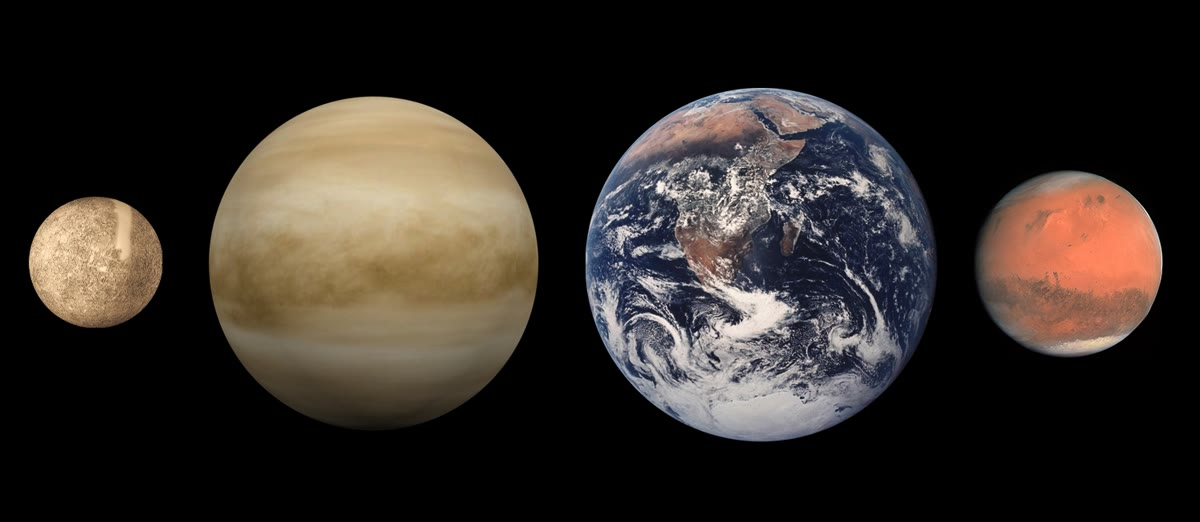
\includegraphics[width=0.85\linewidth]{images/book3/b1-terrestrial-planet-sizes.jpg}

{\small De vier \omterm{def:b1:comparative-planetology:planet-types}{aardachtige planeten} op schaal, van links naar rechts Mercurius,
Venus, de aarde en Mars (afstanden niet op schaal; Venus gezien in zichtbaar licht, haar
oppervlak verborgen onder wolken). NASA, publiek domein.}
% ledger: commons:terrestrial-sizes
\end{omfigure}

\section{Planeten wegen en meten}

De straal van een planeet wordt gemeten uit haar hoekdiameter en haar afstand, of, voor een
planeet die door ruimtevaartuigen is bezocht, uit radar- en lasermetingen van de hoogte. Haar
massa is moeilijker: zij wordt alleen gevoeld door de zwaartekracht die de planeet op iets anders
uitoefent.

\begin{method}[De massa van een planeet uit de baan van een satelliet]\label{met:b1:comparative-planetology:mass}
Voor een satelliet van verwaarloosbare massa in een bijna cirkelvormige baan met straal
(halve lange as) $a$ en siderische omlooptijd $T$ om een planeet met massa $M$:
\begin{enumerate}
  \item reken $a$ om naar meters en $T$ naar seconden;
  \item de derde wet van Kepler geeft $GM = 4\pi^2a^3/T^2$: dit product is wat de baan meet, en
        met veel grotere nauwkeurigheid dan $G$ zelf;
  \item deel door $G = \qty{6.6743e-11}{m^3.kg^{-1}.s^{-2}}$ om $M$ te verkrijgen.
\end{enumerate}
Een planeet zonder maan (Mercurius, Venus) wordt op dezelfde manier gewogen, uit de baan of de
afbuiging van een ruimtevaartuig dat er langs vliegt.
\end{method}

\begin{example}
Io, de binnenste grote maan van Jupiter, draait op $a = \qty{421.8e3}{km}$ in
\num{1.769138} dagen, dat is $T = \qty{152854}{s}$. Dan geldt
\[
  GM = \frac{4\pi^2\times(\qty{4.218e8}{m})^3}{(\qty{152854}{s})^2}
  = \qty{1.268e17}{m^3.s^{-2}}, \qquad
  M = \frac{\num{1.268e17}}{\num{6.6743e-11}} = \qty{1.900e27}{kg},
\]
wat overeenkomt met de getabelleerde massa van Jupiter, \qty{1.898e27}{kg}, tot op
\qty{0.1}{\percent}. De eigen massa van Io, \num{4.7e-5} van die van Jupiter, is verwaarloosbaar;
het kleine overschot komt door de equatoriale uitbolling van Jupiter, die een nabije maan iets
harder trekt dan een bol van dezelfde massa zou doen.
% ledger: nasa:io, nasa:jupiter, const:G
\end{example}

Met massa en straal komt de gemiddelde dichtheid $\bar\rho =
3M/(4\pi R^3)$, de eerste aanwijzing voor waaruit een planeet bestaat. De dichtheden van de
planeten vallen in twee groepen (zie de figuur hieronder): Mercurius, Venus, de aarde en Mars
liggen tussen ongeveer \num{3900} en \qty{5500}{kg.m^{-3}}, dichter dan elk gewoon gesteente; de
vier buitenplaneten liggen tussen \num{690} en \qty{1640}{kg.m^{-3}}, dicht bij die van water,
Saturnus zelfs daaronder.
% ledger: planet:Mercury.density, planet:Mars.density, planet:Earth.density, planet:Saturn.density, planet:Neptune.density

\begin{omfigure}
\begin{tikzpicture}
\begin{axis}[omrecord, width=0.86\linewidth, height=6.2cm, xmode=log,
  xmin=800, xmax=150000, ymin=0, ymax=6300, xlabel={equatoriale straal (km)},
  ylabel={gemiddelde dichtheid (\unit{kg.m^{-3}})}, tick label style={font=\scriptsize},
  label style={font=\small}]
\addplot[only marks, mark=*, mark size=2.4pt, brown!70!black] table[x=R_km, y=density,
  restrict expr to domain={\thisrow{idx}}{0:2}] {figdata/out/bachelor-1-planet_table-bodies.dat};
\addplot[only marks, mark=*, mark size=2.4pt, brown!70!black] table[x=R_km, y=density,
  restrict expr to domain={\thisrow{idx}}{4:4}] {figdata/out/bachelor-1-planet_table-bodies.dat};
\addplot[only marks, mark=*, mark size=2.4pt, orange!85!black] table[x=R_km, y=density,
  restrict expr to domain={\thisrow{idx}}{5:6}] {figdata/out/bachelor-1-planet_table-bodies.dat};
\addplot[only marks, mark=*, mark size=2.4pt, omDef] table[x=R_km, y=density,
  restrict expr to domain={\thisrow{idx}}{7:8}] {figdata/out/bachelor-1-planet_table-bodies.dat};
\addplot[only marks, mark=o, mark size=2.4pt, black!60] table[x=R_km, y=density,
  restrict expr to domain={\thisrow{idx}}{3:3}] {figdata/out/bachelor-1-planet_table-bodies.dat};
\addplot[only marks, mark=o, mark size=2.4pt, black!60] table[x=R_km, y=density,
  restrict expr to domain={\thisrow{idx}}{9:9}] {figdata/out/bachelor-1-planet_table-bodies.dat};
\addplot[black!40, densely dashed] coordinates {(800,1000) (150000,1000)};
\begin{scope}[font=\scriptsize]
\node[left] at (axis cs:2439.5,5429) {Mercurius};
\node[below left] at (axis cs:6052,5243) {Venus};
\node[above] at (axis cs:6378,5514) {aarde};
\node[left] at (axis cs:3396,3934) {Mars};
\node[left] at (axis cs:1737.5,3340) {maan};
\node[right] at (axis cs:1188,1850) {Pluto};
\node[above] at (axis cs:71492,1326) {Jupiter};
\node[left] at (axis cs:60268,687) {Saturnus};
\node[right] at (axis cs:25559,1270) {Uranus};
\node[above] at (axis cs:24764,1638) {Neptunus};
\node[above left, black!60] at (axis cs:150000,1000) {water};
\end{scope}
\end{axis}
\end{tikzpicture}

{\small Gemiddelde dichtheid tegen straal (logaritmisch) voor de acht planeten (gevuld: aardachtig,
\omterm{def:b1:comparative-planetology:planet-types}{gasreuzen}, \omterm{def:b1:comparative-planetology:planet-types}{ijsreuzen}), de maan en Pluto (open cirkels). Gegevens van het planetaire
feitenblad van NASA.}
% ledger: planet:Mercury.diameter, planet:Venus.diameter, planet:Earth.diameter, planet:Moon.diameter, planet:Mars.diameter, planet:Jupiter.diameter, planet:Saturn.diameter, planet:Uranus.diameter, planet:Neptune.diameter, planet:Pluto.diameter, planet:Mercury.density, planet:Venus.density, planet:Earth.density, planet:Moon.density, planet:Mars.density, planet:Jupiter.density, planet:Saturn.density, planet:Uranus.density, planet:Neptune.density, planet:Pluto.density
\end{omfigure}

De gemiddelde dichtheid alleen kan niet onderscheiden tussen een planeet die uit één dicht
materiaal bestaat en een planeet met een zeer dichte kern en een lichtere omhulling. Een tweede
getal doet dat wel: hoe de massa verdeeld is tussen kern en oppervlak.

\begin{definition}[Traagheidsmomentfactor]\label{def:b1:comparative-planetology:moi}
De \emph{traagheidsmomentfactor}\index{traagheidsmomentfactor} van een planeet is het getal
\[
  C = \frac{I}{MR^2} ,
\]
waarin $I$ haar traagheidsmoment om de draaias is, $M$ haar massa en $R$ haar gemiddelde straal.
Een homogene bol heeft $C = \tfrac25 = 0.4$; een planeet waarvan de dichtheid naar het middelpunt
toe toeneemt, heeft $C < 0.4$, des te kleiner naarmate de massa meer naar het midden is
geconcentreerd.
\end{definition}

Het traagheidsmoment wordt gemeten uit de langzame precessie van de draaias onder de aantrekking
van de zon, samen met de afplatting van het zwaartekrachtsveld van de planeet. De waarden zijn
veelzeggend: de maan, $C = 0.394$, is bijna homogeen; Mars, $0.366$, en de aarde, $0.3308$, zijn
duidelijk gelaagd; Jupiter, $0.254$, en Saturnus, $0.210$, hebben het grootste deel van hun massa
naar het midden toe samengepakt.
% ledger: nasa:moon, nasa:mars, earth:MoI, nasa:jupiter, nasa:saturn

\section{Waaruit de planeten bestaan}

\begin{definition}[Aardachtige en reuzenplaneten]\label{def:b1:comparative-planetology:planet-types}
Een \emph{aardachtige planeet}\index{aardachtige planeet} is een planeet die vooral uit silicaatgesteente
en ijzer bestaat, met een vast oppervlak: Mercurius, Venus, de aarde en Mars. Een
\emph{reuzenplaneet}\index{reuzenplaneet} is een planeet die vele malen zwaarder is dan de aarde,
vooral uit lichte elementen en hun verbindingen bestaat en geen vast oppervlak heeft. Een
\emph{gasreus}\index{gasreus} is een reuzenplaneet die vooral uit waterstof en helium bestaat:
Jupiter en Saturnus. Een \emph{ijsreus}\index{ijsreus} is een reuzenplaneet die vooral uit de
verbindingen bestaat die sterrenkundigen ijzen noemen --- water, methaan en ammoniak --- onder
een omhulling van waterstof en helium: Uranus en Neptunus.
\end{definition}

De atmosferen die sondes en telescopen meten, bevestigen de indeling. Die van Jupiter bestaat voor
\qty{89.8}{\percent} uit waterstof en \qty{10.2}{\percent} uit helium naar volume, die van Saturnus
voor \qty{96.3}{\percent} en \qty{3.25}{\percent}; voor Uranus is ten minste \qty{80}{\percent} van de
massa een hete dichte vloeistof van water, methaan en ammoniak boven een kleine rotskern. De gemiddelde
dichtheid van een \omterm{def:b1:comparative-planetology:planet-types}{gasreus} blijft laag, hoewel haar middelpunt sterk is samengedrukt, omdat waterstof het
lichtste element is; een \omterm{def:b1:comparative-planetology:planet-types}{ijsreus} is dichter dan Saturnus omdat haar ijzen zwaarder zijn dan waterstof.
% ledger: nasa:jupiter, nasa:saturn, nasa:uranus-structure

De \omterm{def:b1:comparative-planetology:planet-types}{aardachtige planeten} zijn gelaagd zoals de aarde: een ijzerrijke kern onder een silicaatmantel en
een dunne korst. Het eenvoudigste model dat beide gemeten getallen gebruikt, de gemiddelde dichtheid
en de \omterm{def:b1:comparative-planetology:moi}{traagheidsmomentfactor}, heeft twee lagen.

\begin{proposition}[De planeet met twee lagen]\label{prop:b1:comparative-planetology:two-layer}
Beschouw een planeet met straal $R$ als een kern met straal $xR$ en homogene dichtheid $\rho_c$
binnen een mantel met homogene dichtheid $\rho_m$. Haar gemiddelde dichtheid en haar
\omterm{def:b1:comparative-planetology:moi}{traagheidsmomentfactor} zijn
\[
  \bar\rho = \rho_m + (\rho_c - \rho_m)\,x^3 , \qquad
  C = \frac25\,\frac{\rho_m + (\rho_c - \rho_m)\,x^5}{\bar\rho} .
\]
Gegeven $\bar\rho$, $C$ en een aangenomen dichtheid van de mantel $\rho_m$, volgt de relatieve
straal van de kern:
\[
  x^2 = \frac{\tfrac52C\bar\rho - \rho_m}{\bar\rho - \rho_m} ,
  \qquad \rho_c = \rho_m + \frac{\bar\rho - \rho_m}{x^3} .
\]
\end{proposition}

\begin{proof}
De planeet is een homogene bol met dichtheid $\rho_m$ en straal $R$ plus een bol met straal $xR$ en
het overschot aan dichtheid $\rho_c - \rho_m$. Massa's tellen op:
$M = \tfrac43\pi R^3[\rho_m + (\rho_c - \rho_m)x^3]$, en delen door het volume geeft $\bar\rho$.
Traagheidsmomenten om dezelfde as tellen ook op; een homogene bol met dichtheid $\rho$ en straal $r$ heeft
$I = \tfrac25\cdot\tfrac43\pi\rho r^3\cdot r^2 = \tfrac{8\pi}{15}\rho r^5$, dus
$I = \tfrac{8\pi}{15}R^5[\rho_m + (\rho_c - \rho_m)x^5]$. Delen door
$MR^2 = \tfrac43\pi\bar\rho R^5$ geeft $C$. Ten slotte luiden de twee vergelijkingen
$(\rho_c - \rho_m)x^3 = \bar\rho - \rho_m$ en $(\rho_c - \rho_m)x^5 =
\tfrac52C\bar\rho - \rho_m$; delen van de tweede door de eerste geeft $x^2$, en de eerste
geeft $\rho_c$.
\end{proof}

Het model heeft drie onbekenden en twee gegevens, dus één ervan, de dichtheid van de mantel, moet
worden aangenomen uit wat gesteenten van de juiste samenstelling onder druk wegen. Het antwoord is
gevoelig voor die keuze wanneer $C$ dicht bij $0.4$ ligt, omdat $\tfrac52C\bar\rho - \rho_m$ dan een
klein verschil van grote getallen is (\cref{exo:b1:comparative-planetology:10} en het probleem). Het
model negeert ook de samendrukking van de mantel door haar eigen gewicht, die in een planeet zo groot
als de aarde de dichtheid van de diepe mantel ver boven die van oppervlaktegesteenten opvoert; voor
de aarde doet de seismologie het veel beter (\cref{ch:b1:layered-earth}). Seismometers op Mars doen
dat nu ook voor die planeet: waar de planetaire tabel een kernstraal van \qty{1830}{km}
geeft, wijzen recente resultaten op slechts \qty{1650}{km} tot \qty{1675}{km}.
% ledger: nasa:mars-core

\begin{omfigure}
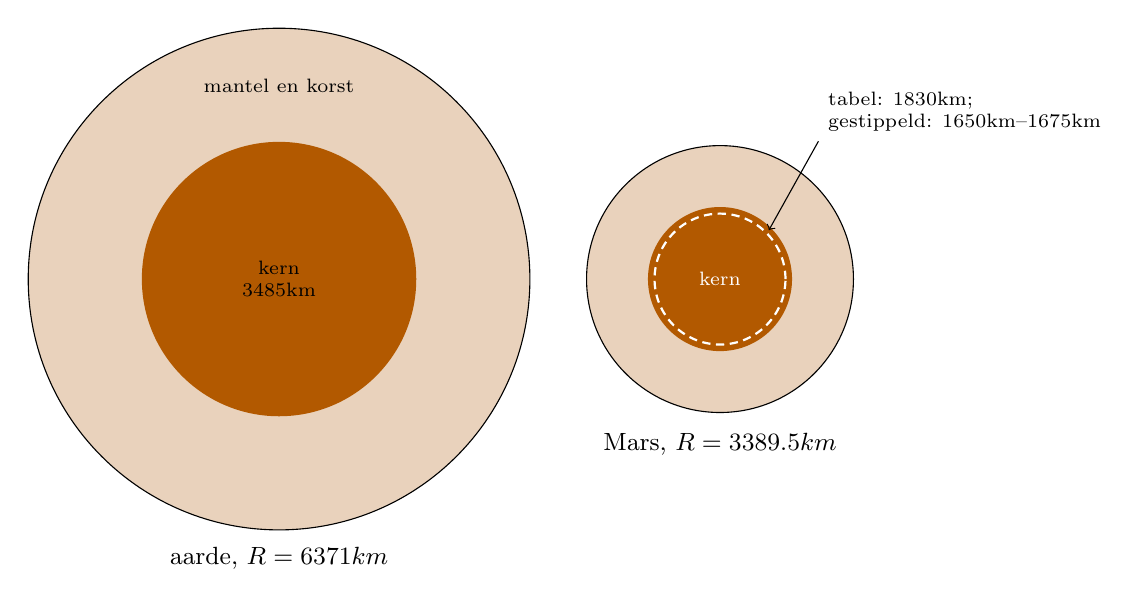
\begin{tikzpicture}[font=\scriptsize]
% scale: 0.5 cm per 1000 km
\fill[brown!35] (0,0) circle (3.1855cm);
\fill[orange!70!black] (0,0) circle (1.7425cm);
\draw (0,0) circle (3.1855cm);
\node[align=center] at (0,0) {kern\\ \qty{3485}{km}};
\node[align=center] at (0,2.45) {mantel en korst};
\node at (0,-3.55) {\small aarde, $R = \qty{6371}{km}$};
\begin{scope}[xshift=5.6cm]
\fill[brown!35] (0,0) circle (1.6948cm);
\fill[orange!70!black] (0,0) circle (0.915cm);
\draw[white, densely dashed, thick] (0,0) circle (0.8313cm);
\draw (0,0) circle (1.6948cm);
\node[align=center, white] at (0,0) {kern};
\node at (0,-2.1) {\small Mars, $R = \qty{3389.5}{km}$};
\draw[->] (1.25,1.75) node[above right, align=left] {tabel: \qty{1830}{km};\\ gestippeld: \qty{1650}{km}--\qty{1675}{km}} -- (0.62,0.62);
\end{scope}
\end{tikzpicture}

{\small De aarde en Mars op schaal, met hun kernen. Voor Mars is de vaste rand de kernstraal van de
planetaire tabel en de gestippelde cirkel de kleinere straal die recente seismische resultaten
aangeven. Beide kernen zijn ijzerrijk; de kern van de aarde heeft een vast binnendeel, dat niet is
getekend.}
% ledger: earth:Rmean, earth:Rcore, nasa:mars, nasa:mars-core
\end{omfigure}

\section{Atmosferen en oppervlakken}

De temperatuur van een planeet wordt eerst bepaald door het zonlicht dat zij absorbeert. De
instraling $S$ op haar afstand $d$ van de zon neemt af als $1/d^2$
(\cref{prop:b1:observing-the-sky:inverse-square}): \qty{1361}{W.m^{-2}} bij de aarde,
\qty{2601}{W.m^{-2}} bij Venus, \qty{586}{W.m^{-2}} bij Mars, \qty{50}{W.m^{-2}} bij Jupiter.
Een deel ervan wordt direct weer teruggekaatst.
% ledger: earth:TSI, nasa:venus, nasa:mars, nasa:jupiter

\begin{definition}[Bond-albedo]\label{def:b1:comparative-planetology:albedo}
Het \emph{Bond-albedo}\index{Bond-albedo} $A$ van een planeet is het deel van het totale vermogen van
het zonlicht dat op haar valt, dat zij terugkaatst en naar de ruimte verstrooit, over alle golflengten
en alle richtingen.
\end{definition}

Vers sneeuw en heldere wolken kaatsen veel terug, donker gesteente en open zee weinig. Venus, in heldere
wolken gehuld, heeft $A = 0.77$; de aarde $0.294$; Mars $0.250$; de maan, donkergrijs gesteente, $0.11$.
% ledger: nasa:venus, earth:albedo, nasa:mars, nasa:moon

\begin{definition}[Evenwichtstemperatuur]\label{def:b1:comparative-planetology:equilibrium-temperature}
De \emph{evenwichtstemperatuur}\index{evenwichtstemperatuur} $T_\mathrm{eq}$ van een planeet is de
uniforme temperatuur waarop een zwart lichaam van de grootte van de planeet precies het vermogen naar de
ruimte zou uitstralen dat de planeet van de zon absorbeert.
\end{definition}

\begin{proposition}[Evenwichtstemperatuur]\label{prop:b1:comparative-planetology:teq}
Een planeet met \omterm{def:b1:comparative-planetology:albedo}{Bond-albedo} $A$ die de instraling $S$ ontvangt, heeft
\[
  T_\mathrm{eq} = \left(\frac{S(1 - A)}{4\sigma}\right)^{1/4},
  \qquad \sigma = \qty{5.6704e-8}{W.m^{-2}.K^{-4}} .
\]
\end{proposition}

\begin{proof}
De planeet vangt het zonlicht op dat op haar dwarsdoorsnede valt, een schijf met oppervlak $\pi R^2$,
en absorbeert het deel $1 - A$: zij absorbeert $S(1 - A)\pi
R^2$. Een zwart lichaam (de wet van
Stefan--Boltzmann, die uit het tweede jaar van de natuurkundeboeken wordt overgenomen) met uniforme
temperatuur $T$ straalt $\sigma T^4$ uit van elke vierkante meter van zijn hele oppervlak, $4\pi R^2$.
Met de twee vermogens aan elkaar gelijk: $4\pi R^2\sigma T^4 = S(1 - A)\pi R^2$, en de factor 4 is de
verhouding van het oppervlak van de bol tot haar dwarsdoorsnede.
\end{proof}

Met de bovenstaande waarden is $T_\mathrm{eq}$ \qty{255}{K} voor de aarde, \qty{227}{K} voor Venus,
\qty{210}{K} voor Mars en \qty{270}{K} voor de maan. Venus komt, hoewel dichter bij de zon, kouder
uit dan de aarde: haar wolken kaatsen driekwart van het zonlicht terug. De figuur hieronder zet deze
waarden naast de gemeten gemiddelde oppervlaktetemperaturen. De verschillen zijn het broeikaseffect,
dat de volgende alinea's en de klimaathoofdstukken (\cref{ch:b1:radiation-heat-transport}) kwantitatief
maken: ongeveer \qty{33}{K} voor de aarde, ongeveer \qty{510}{K} voor Venus, slechts ongeveer
\qty{4}{K} voor Mars.
% ledger: const:sigma, earth:Tsurf, nasa:venus, nasa:mars, planet:Moon.Tmean

\begin{omfigure}
\begin{tikzpicture}
\begin{axis}[ybar, bar width=12pt, width=0.72\linewidth, height=5.8cm,
  ymin=0, ymax=820, xmin=-0.6, xmax=3.6, xtick={0,1,2,3},
  xticklabels={maan, Mars, aarde, Venus}, ylabel={temperatuur (K)},
  tick label style={font=\scriptsize}, label style={font=\small},
  ymajorgrids, grid style={black!12}, axis lines*=left,
  legend style={font=\scriptsize, at={(0.03,0.97)}, anchor=north west, draw=none},
  nodes near coords, nodes near coords style={font=\tiny},
  every node near coord/.append style={/pgf/number format/fixed, /pgf/number format/precision=0}]
\addplot[fill=omDef!55, draw=omDef] table[x=idx, y=Teq] {figdata/out/bachelor-1-planet_table-temps.dat};
\addplot[fill=omThm!60, draw=omThm] table[x=idx, y=Tsurf] {figdata/out/bachelor-1-planet_table-temps.dat};
\legend{evenwichtstemperatuur, gemiddelde oppervlaktetemperatuur}
\end{axis}
\end{tikzpicture}

{\small \omterm{def:b1:comparative-planetology:equilibrium-temperature}{Evenwichtstemperatuur} (berekend uit de instraling en het \omterm{def:b1:comparative-planetology:albedo}{Bond-albedo}) en gemeten gemiddelde
oppervlaktetemperatuur van vier lichamen. De atmosfeer verwarmt de aarde en vooral Venus; de dunne
atmosfeer van Mars doet weinig; de ijle maan is gemiddeld kouder dan haar \omterm{def:b1:comparative-planetology:equilibrium-temperature}{evenwichtstemperatuur}.}
% ledger: nasa:moon, nasa:mars, earth:TSI, earth:albedo, earth:Tsurf, nasa:venus, planet:Moon.Tmean, const:sigma
\end{omfigure}

De gemiddelde temperatuur van de maan, ongeveer \qty{253}{K}, ligt onder haar \omterm{def:b1:comparative-planetology:equilibrium-temperature}{evenwichtstemperatuur}.
Dat is geen paradox: zonder atmosfeer of oceaan om warmte te vervoeren, is de dagzijde zeer heet en de
nachtzijde zeer koud, en omdat de uitstraling met $T^4$ groeit, straalt een lichaam met ongelijke
temperaturen de geabsorbeerde energie uit bij een lagere gemiddelde temperatuur dan een uniform
lichaam (\cref{exo:b1:comparative-planetology:11}).

Een atmosfeer doet twee dingen: zij laat het meeste zonlicht door en zij absorbeert een deel van de
infrarode straling die de bodem uitzendt, en straalt een deel ervan naar beneden terug. Hoeveel zij het
oppervlak verwarmt, hangt af van hoeveel absorberend gas erboven ligt op elke vierkante meter. De
oppervlaktedruk meet precies dat: $p = mg$ voor een kolom van massa $m$ per vierkante meter. De atmosfeer
van Venus, bij \qty{92}{bar}, bestaat voor \qty{96.5}{\percent} uit koolstofdioxide; die van Mars, met
slechts \qty{6.36}{mbar} gemiddeld, bestaat ook voor \qty{95.1}{\percent} uit koolstofdioxide, maar bevat
boven elke vierkante meter ongeveer zestig keer minder gas dan die van de aarde, en zeer weinig waterdamp.
Beide planeten hebben koolstofdioxideatmosferen; slechts één ervan heeft een dikke.
% ledger: nasa:venus, nasa:mars, earth:psurf

\begin{omfigure}
\begin{minipage}{0.4\linewidth}
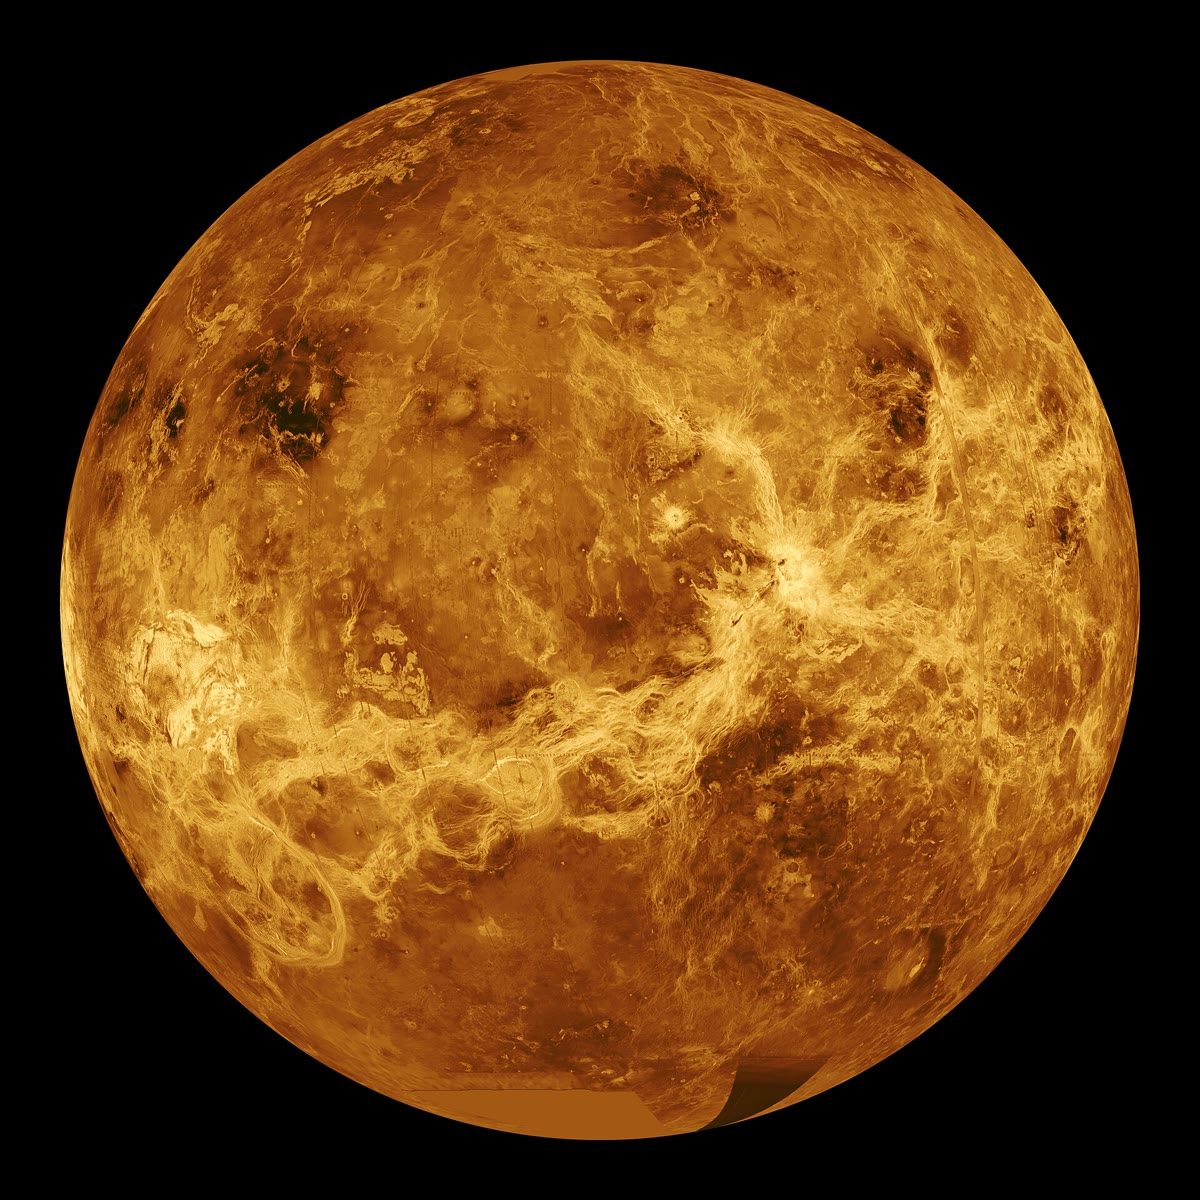
\includegraphics[width=\linewidth]{images/book3/b1-venus-radar-globe.jpg}
\end{minipage}\hspace{0.06\linewidth}
\begin{minipage}{0.4\linewidth}
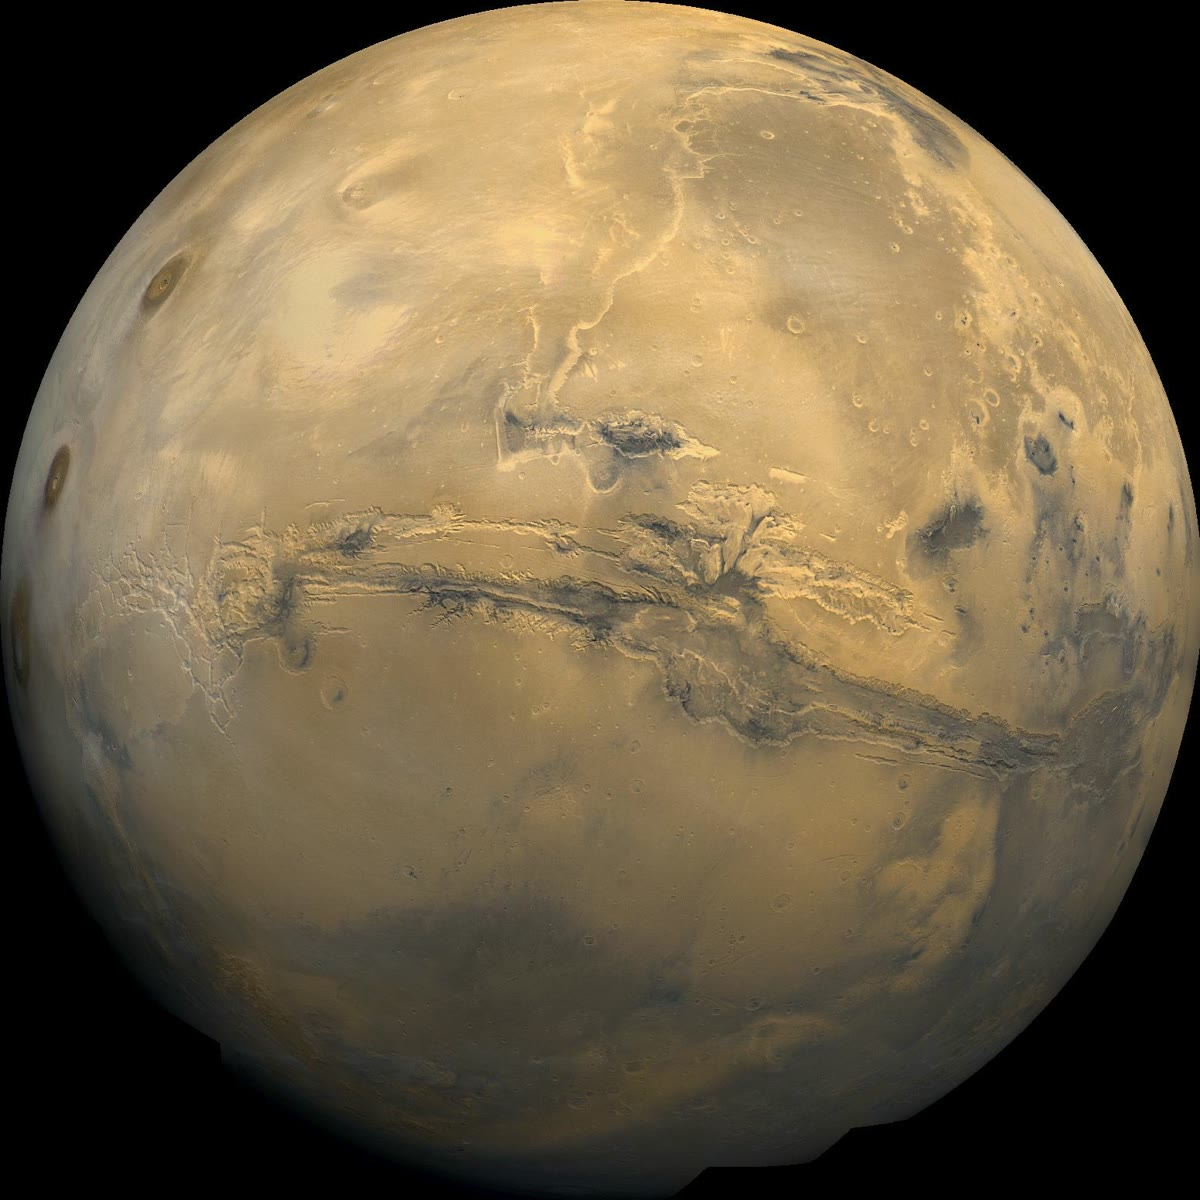
\includegraphics[width=\linewidth]{images/book3/b1-mars-valles-marineris.jpg}
\end{minipage}

{\small Links: het oppervlak van Venus, gezien door de wolken met de radar van de ruimtesonde Magellan,
op een computergesimuleerde bol aangebracht (de kleuren zijn gesimuleerd). Rechts: Mars van de baan van
Viking 1, een mozaïek gecentreerd op het canyonsysteem van Valles Marineris. NASA/JPL en NASA/USGS,
publiek domein.}
% ledger: commons:venus-globe, commons:mars-valles
\end{omfigure}

De oppervlakken dragen het bewijs van wat hen heeft gevormd. Inslagkraters hopen zich op aan elk oppervlak
dat aan de ruimte is blootgesteld, dus een zwaar bekraterd oppervlak, zoals het grootste deel van de maan
of van Mercurius, is oud, en een oppervlak met weinig kraters is vernieuwd: door lavastromen, door erosie,
of door de platen die de oceaanbodem van de aarde terug in de mantel voeren. Vulkanische vlakten en vulkanen
komen op alle \omterm{def:b1:comparative-planetology:planet-types}{aardachtige planeten} voor. Breuken, slenken en geplooide gordels tonen aan dat de lithosferen
van Venus en Mars zijn vervormd; maar van alle planeten vertoont alleen de aarde vandaag een lithosfeer die in
platen is gebroken die als starre blokken bewegen, met ruggen waar zij worden gevormd en troggen waar zij
zinken. Waarom alleen de aarde platentektoniek heeft, wordt nog besproken; de aanwezigheid van water, dat
gesteenten verzwakt, is een van de redenen die worden aangevoerd.

\section{Manen en kleine lichamen}

De maan, een kwart van de diameter van de aarde, is groot voor een satelliet. Haar dichtheid,
\qty{3340}{kg.m^{-3}}, dicht bij die van de gesteenten van de aardmantel, en haar
\omterm{def:b1:comparative-planetology:moi}{traagheidsmomentfactor}, dicht bij $0.4$, tonen aan dat zij hooguit een kleine ijzeren kern heeft. De \omterm{def:b1:comparative-planetology:planet-types}{reuzenplaneten}
hebben stelsels van manen die op zichzelf werelden zijn (zie de foto's hieronder). Io, de binnenste van
Jupiters vier grote manen, is de meest vulkanisch actieve wereld van het zonnestelsel, met honderden vulkanen,
verwarmd door de getijden die Jupiter in haar opwekt; het vulkanisme vernieuwt haar oppervlak sneller dan
inslagen met grote kraters het kunnen merken. Europa, met een dichtheid van \qty{3010}{kg.m^{-3}}, bestaat uit
gesteente onder een korst van ijs, en er zijn sterke aanwijzingen voor een zoute oceaan onder die korst.
Ganymedes en Callisto, met dichtheden van \num{1940} en \qty{1830}{kg.m^{-3}}, bestaan uit gesteente en ijs
in vergelijkbare hoeveelheden.
Titan, de grootste maan van Saturnus, is de enige maan met een dichte atmosfeer, vooral uit stikstof met een
beetje methaan, en de enige wereld naast de aarde met rivieren, meren en zeeën op het oppervlak --- van vloeibaar
methaan en ethaan; ook zij verbergt waarschijnlijk een oceaan van water.
% ledger: planet:Moon.diameter, planet:Earth.diameter, planet:Moon.density, nasa:moon, nasa:io-facts, nasa:europa, nasa:europa-facts, nasa:ganymede, nasa:titan-facts

\begin{omfigure}
\begin{minipage}{0.4\linewidth}
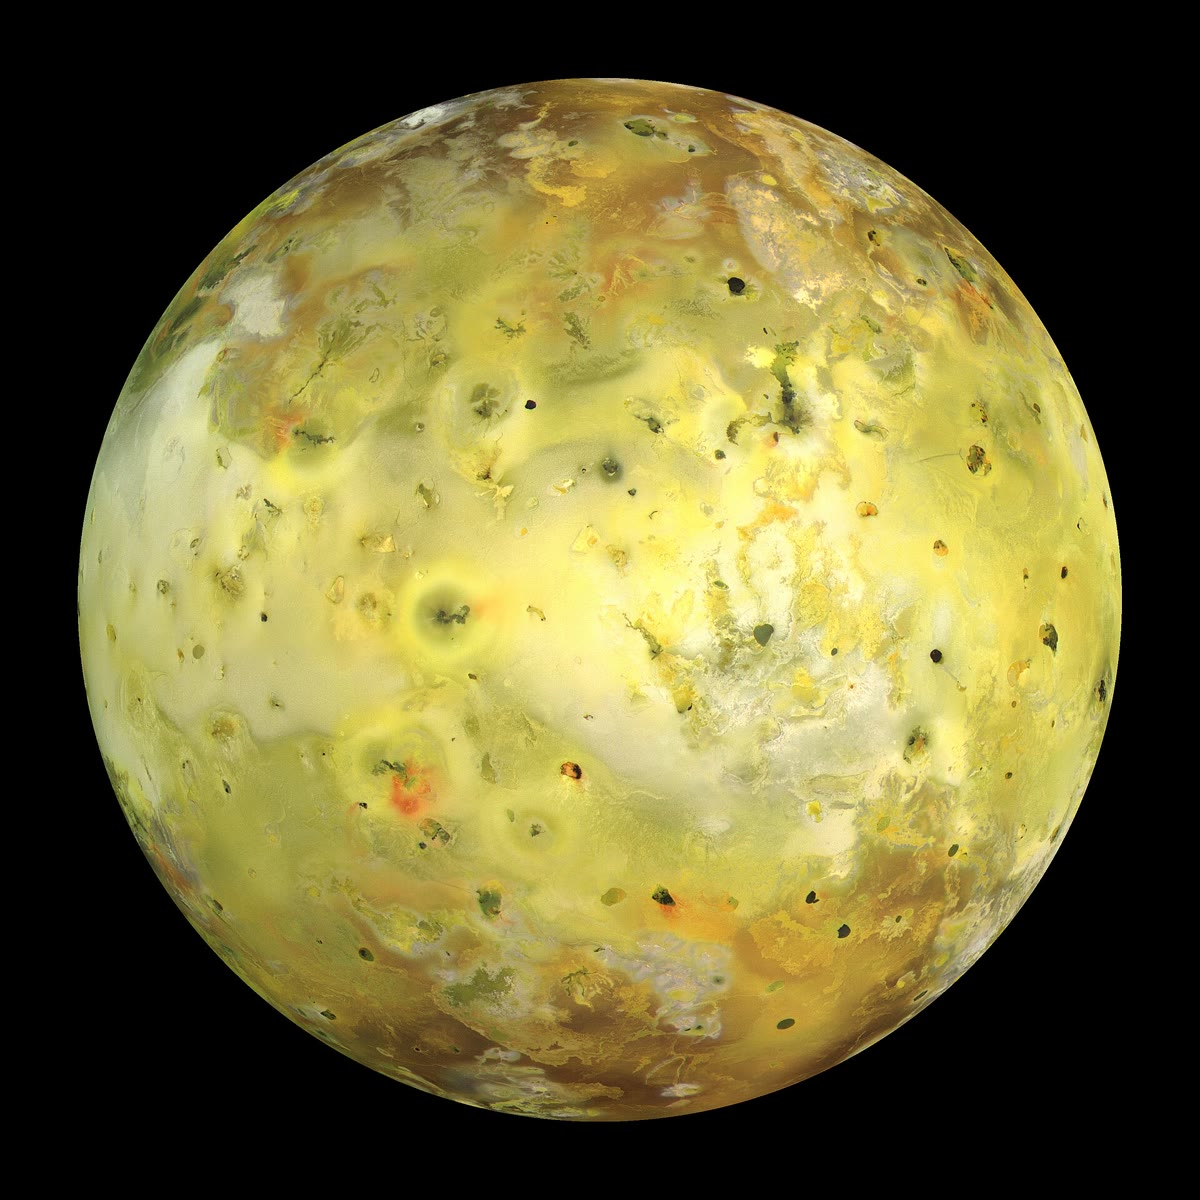
\includegraphics[width=\linewidth]{images/book3/b1-io.jpg}
\end{minipage}\hspace{0.06\linewidth}
\begin{minipage}{0.4\linewidth}
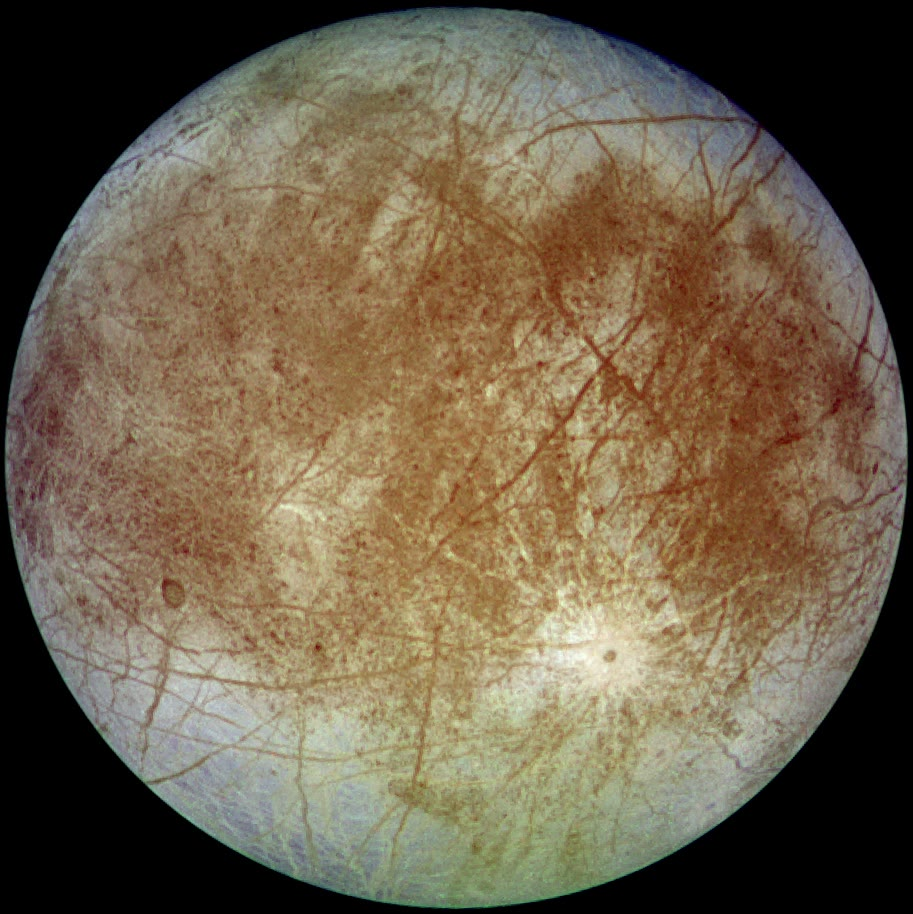
\includegraphics[width=\linewidth]{images/book3/b1-europa.jpg}
\end{minipage}

{\small Twee grote manen van Jupiter, gezien door de ruimtesonde Galileo. Links: Io, haar oppervlak bezaaid met
vulkanische centra en gekleurd door zwavelverbindingen en lavas. Rechts: Europa in benaderde natuurlijke kleur;
de lange donkere lijnen zijn breuken in haar ijskorst. NASA/JPL/University of Arizona en NASA/JPL/DLR, publiek domein.}
% ledger: commons:io, commons:europa, nasa:io-facts, nasa:europa
\end{omfigure}

\begin{definition}[Planetoïde, komeet, trans-Neptunisch object]\label{def:b1:comparative-planetology:small-bodies}
Een \emph{planetoïde}\index{planetoïde} is een klein rotsachtig of metallisch lichaam dat om de zon draait, te klein
om een planeet te zijn en zonder de gas- en stofomhulling van een komeet; de meeste draaien tussen Mars en Jupiter.
Een \emph{komeet}\index{komeet} is een klein lichaam van ijs en stof dat, wanneer zijn baan het dicht bij de zon
brengt, gas en stof vrijgeeft die rond hem een gloeiende omhulling vormen en staarten die van de zon af wijzen. Een
\emph{trans-Neptunisch object}\index{trans-Neptunisch object} is een lichaam van het zonnestelsel waarvan de baan
gemiddeld voorbij die van Neptunus ligt.
\end{definition}

De trans-Neptunische objecten van de Kuipergordel, een schijfvormige zone voorbij Neptunus, zijn ijzige en
rotsachtige lichamen die zijn overgebleven van de vorming van de planeten; Pluto, sinds 2006 als dwergplaneet
aangemerkt, is er een van. De \omterm{def:b1:comparative-planetology:small-bodies}{planetoïden} zijn het puin van een gebied waar geen planeet is gevormd. Stukken
\omterm{def:b1:comparative-planetology:small-bodies}{planetoïden}, en een paar van de maan en van Mars, vallen als meteorieten op de aarde. Zij zijn, naast de
monsters die door ruimtevaartuigen zijn teruggebracht, de enige monsters van andere werelden die wij in handen
hebben; sommige ervan zijn sinds de vorming van het zonnestelsel nauwelijks veranderd. Hun klassen, en wat zij
zeggen over de samenstelling van de aarde en de leeftijd van het zonnestelsel, zijn het onderwerp van Boek 4.
% ledger: nasa:pluto-facts

\section{Oefeningen}

\begin{exercise}[$\star$]\label{exo:b1:comparative-planetology:1}
Jupiter heeft een massa van \qty{1898.13e24}{kg} en een gemiddelde straal van \qty{69911}{km}. Bereken
haar gemiddelde dichtheid en vergelijk die met die van water, \qty{1000}{kg.m^{-3}}.
\end{exercise}

\begin{exercise}[$\star$]\label{exo:b1:comparative-planetology:2}
Classificeer aan de hand van de figuur van dichtheden en stralen Mercurius, Saturnus, Uranus en Venus als
\omterm{def:b1:comparative-planetology:planet-types}{aardachtige planeten}, \omterm{def:b1:comparative-planetology:planet-types}{gasreuzen} of \omterm{def:b1:comparative-planetology:planet-types}{ijsreuzen}, en onderbouw elke keuze met hun straal en dichtheid.
\end{exercise}

\begin{exercise}[$\star$]\label{exo:b1:comparative-planetology:3}
Venus ontvangt \qty{2601.3}{W.m^{-2}} en heeft een \omterm{def:b1:comparative-planetology:albedo}{Bond-albedo} van 0.77. Bereken haar \omterm{def:b1:comparative-planetology:equilibrium-temperature}{evenwichtstemperatuur}.
Waarom is zij lager dan die van de aarde, hoewel Venus dichter bij de zon staat?
\end{exercise}

\begin{exercise}[$\star$]\label{exo:b1:comparative-planetology:4}
Rangschik de maan ($C = 0.394$), Mars (0.366), de aarde (0.3308), Jupiter (0.254) en Saturnus (0.210) van het
meest homogene naar het meest centraal geconcentreerde. Hoe groot zou $C$ zijn voor een planeet waarvan de
hele massa in een punt in het middelpunt zit?
\end{exercise}

\begin{exercise}[$\star\star$]\label{exo:b1:comparative-planetology:5}
Titan draait om Saturnus op $a = \qty{1221.87e3}{km}$ in \num{15.945421} dagen. Bereken de massa van Saturnus en
vergelijk die met de getabelleerde \qty{568.32e24}{kg}.
\end{exercise}

\begin{exercise}[$\star\star$]\label{exo:b1:comparative-planetology:6}
De aarde ontvangt \qty{1361}{W.m^{-2}} op \qty{149.6e6}{km} van de zon. Bereken de instraling bij Mars
(\qty{228.0e6}{km}) en bij Jupiter (\qty{778.5e6}{km}), en vergelijk met de getabelleerde \qty{586.2}{W.m^{-2}}
en \qty{50.26}{W.m^{-2}}.
\end{exercise}

\begin{exercise}[$\star\star$]\label{exo:b1:comparative-planetology:7}
Toon aan dat $T_\mathrm{eq}$ voor een gegeven albedo varieert als $d^{-1/2}$. Bereken $T_\mathrm{eq}$ voor Jupiter
($S = \qty{50.26}{W.m^{-2}}$, $A = 0.343$). Als men zou vinden dat Jupiter meer vermogen uitstraalt dan het
van de zon absorbeert, wat zou dat dan zeggen over haar binnenste?
\end{exercise}

\begin{exercise}[$\star\star$]\label{exo:b1:comparative-planetology:8}
Bereken het broeikasopwarmingseffect $T_\mathrm{oppervlak} - T_\mathrm{eq}$ van Venus (\qty{737}{K}), de aarde
(\qty{288}{K}, $A = 0.294$) en Mars (\qty{214}{K}). Druk elk uit als een fractie van $T_\mathrm{eq}$.
\end{exercise}

\begin{exercise}[$\star\star$]\label{exo:b1:comparative-planetology:9}
Toon voor een homogene bol aan dat $C = 0.4$ door de traagheidsmomenten van dunne bolschillen te integreren (een
schil met straal $r$ en massa $\mathrm dm$ heeft $\mathrm dI = \tfrac23 r^2\,\mathrm dm$). Welke waarde heeft een
holle bolschil met straal $R$?
\end{exercise}

\begin{exercise}[$\star\star\star$]\label{exo:b1:comparative-planetology:10}
Mercurius heeft $\bar\rho = \qty{5429}{kg.m^{-3}}$, $C = 0.35$ en een straal van \qty{2439.7}{km}. Met een
dichtheid van de mantel van \qty{3300}{kg.m^{-3}} gebruikt men het model met twee lagen om haar kernstraal, haar
kerndichtheid en de massafractie van de kern te vinden. Wat is opmerkelijk aan Mercurius?
\end{exercise}

\begin{exercise}[$\star\star\star$]\label{exo:b1:comparative-planetology:11}
Modelleer een lichaam zonder atmosfeer waarvan de dagzijde op de uniforme temperatuur $T_1$ ligt en de nachtzijde op
$T_2$, die samen de geabsorbeerde energie uitstralen. (a) Toon aan dat als $T_1^4 + T_2^4 = 2T_\mathrm{eq}^4$, de
gemiddelde temperatuur $(T_1 + T_2)/2$ hooguit $T_\mathrm{eq}$ is, met gelijkheid alleen wanneer $T_1 = T_2$. (b) Voor de
maan is $T_\mathrm{eq} = \qty{270}{K}$; neem $T_2 = \qty{100}{K}$. Bereken $T_1$ en de gemiddelde temperatuur.
\end{exercise}

\begin{exercise}[$\star\star\star$]\label{exo:b1:comparative-planetology:12}
Venus heeft een straal van \qty{6051.8}{km}, een oppervlaktezwaartekracht van \qty{8.9}{m.s^{-2}} en een
oppervlaktedruk van \qty{92}{bar}. Bereken de massa van haar atmosfeer, vergelijk die met die van de aarde,
\qty{5.1e18}{kg}, en met de massa van Venus, \qty{4.8673e24}{kg}. Wat suggereert de vergelijking over waar de
koolstofdioxide van de aarde is opgeslagen?
% ledger: earth:Matm, planet:Venus.gravity, nasa:venus
\end{exercise}

\section{Probleem: Mars wegen en doorgronden}

\begin{problem}[{Weekendprobleem --- de massa van Mars uit haar maan, haar dichtheid en temperatuur, en de grootte van haar kern}]
\label{pb:b1:comparative-planetology:1}
% ledger: nasa:phobos, nasa:mars, nasa:mars-core, const:G, const:sigma, earth:psurf, earth:gmean, planet:Mars.Prot, planet:Earth.density
% numbers computed in the scratch calculator calc/ch03.py from the rounded data
Fobos, de grotere maan van Mars, draait op een gemiddelde afstand van \qty{9378}{km} van het middelpunt van Mars in
\num{0.31891} dagen. Mars heeft een gemiddelde straal van \qty{3389.5}{km}, een rotatieperiode van \qty{24.6}{h}, een
\omterm{def:b1:comparative-planetology:moi}{traagheidsmomentfactor} $C = 0.366$, een \omterm{def:b1:comparative-planetology:albedo}{Bond-albedo} van 0.250 en een gemiddelde oppervlaktedruk van \qty{6.36}{mbar};
zij ontvangt \qty{586.2}{W.m^{-2}} van de zon, en haar gemiddelde oppervlaktetemperatuur is ongeveer \qty{214}{K}.
Fobos heeft een massa van \qty{1.06e16}{kg}. Neem $G = \qty{6.6743e-11}{m^3.kg^{-1}.s^{-2}}$ en
$\sigma = \qty{5.6704e-8}{W.m^{-2}.K^{-4}}$.

\medskip
\noindent\textbf{Deel I --- Mars wegen.}
\begin{enumerate}
  \item Reken de omlooptijd van Fobos om naar seconden.
  \item Bereken $GM$ voor Mars.
  \item Leid de massa van Mars af.
  \item Is het juist de massa van Fobos te verwaarlozen?
  \item Bereken de baansnelheid van Fobos.
  \item Vergelijk de omlooptijd van Fobos met de rotatie van Mars. In welke richting kruist Fobos de hemel van Mars?
\end{enumerate}

\medskip
\noindent\textbf{Deel II --- Dichtheid en zwaartekracht.}
\begin{enumerate}[resume]
  \item Bereken het volume van Mars.
  \item Bereken haar gemiddelde dichtheid, afgerond op \qty{10}{kg.m^{-3}}.
  \item Vergelijk die met die van de aarde, \qty{5514}{kg.m^{-3}}. Geef twee redenen waarom de aarde dichter is.
  \item Bereken de zwaartekracht aan het oppervlak van Mars.
  \item Bereken de ontsnappingssnelheid vanaf het oppervlak van Mars.
\end{enumerate}

\medskip
\noindent\textbf{Deel III --- Temperatuur en atmosfeer.}
\begin{enumerate}[resume]
  \item Bereken de \omterm{def:b1:comparative-planetology:equilibrium-temperature}{evenwichtstemperatuur} van Mars.
  \item Vergelijk die met de gemiddelde oppervlaktetemperatuur. Hoe groot is het broeikasopwarmingseffect?
  \item Bereken de massa van de atmosfeer boven elke vierkante meter van Mars, en vergelijk die met de aarde ($p = \qty{1014}{hPa}$,
        $g = \qty{9.82}{m.s^{-2}}$).
  \item Bereken de totale massa van de atmosfeer van Mars.
  \item De atmosfeer van Mars bestaat voor \qty{95}{\percent} uit koolstofdioxide, toch is haar broeikasopwarming klein. Geef een
        verklaring.
\end{enumerate}

\medskip
\noindent\textbf{Deel IV --- De kern van Mars.}
\begin{enumerate}[resume]
  \item Hoe groot zou $C$ zijn als Mars homogeen was? Wat zegt de gemeten waarde?
  \item Schrijf de gemiddelde dichtheid van een tweelagige Mars uit in termen van de relatieve kernstraal $x$, de mantelsdichtheid $\rho_m$ en de kerndichtheid $\rho_c$.
  \item Schrijf haar \omterm{def:b1:comparative-planetology:moi}{traagheidsmomentfactor} uit in dezelfde termen.
  \item Toon aan dat $x^2 = (\tfrac52C\bar\rho - \rho_m)/(\bar\rho - \rho_m)$.
  \item Met de gemiddelde dichtheid uit vraag 8 en $\rho_m =
        \qty{3500}{kg.m^{-3}}$, bereken $x$ en de kerndichtheid.
  \item Welk deel van de massa van Mars zit in haar kern?
  \item Herhaal vraag 21 met $\rho_m = 3450$ en \qty{3550}{kg.m^{-3}}. Welke conclusie volgt over de nauwkeurigheid van het model?
  \item Geef de straal van de kern van Mars uit het model met $\rho_m = \qty{3500}{kg.m^{-3}}$, en vergelijk die met de waarde van de planetaire tabel, \qty{1830}{km}, en met het recente seismische resultaat, \qty{1650}{km} tot \qty{1675}{km}.
\end{enumerate}
\end{problem}
